\section{Experimentacion General}
En esta secci\'on analizaremos la calidad de las heuristicas mediante la comparaci\'on y analisis estadistico de las soluciones, asi tambien el tiempo insumido en obtener dichas soluciones, para diferentes grupos de instancias de grafos generados al azar.

\subsection{Generacion de conjuntos de grafos aleatorios}

\subsubsection{Generador de grafos aleatorios}
El generador aleatorio de grafos es un binario aparte de los algoritmos, que recibe como parametros

\begin{itemize}
	\item cantidad de nodos
	\item cantidad de aristas
	\item peso maximo $w_1$
	\item peso maximo $w_2$
	\item limite $w_1$
\end{itemize}

y devuelve por salida estandar una instancia del problema tal como esta especificado el formato de entrada en el enunciado de este TP.\\

\textbf{Nota: }Los generadores de numeros aleatorios de este generador de grafos tienen distribucion uniforme(Usan random de C++11).\\

La generaci\'on del grafo se realiza de la siguiente manera:\\
Se eligen al azar, los nodos de origen y destino, con distribucion uniforme en el rango correspondiente a los numeros que identifican nodos en el grafo. Acto seguido se imprime la linea de cabecera a la salida estandar con todos los datos correspondientes.\\
Para la generacion de las aristas.
\vspace{3cm}






			NICO: TODOOOOOOOOOOOOOOO!!!!!!!!!!!!!!!!

\vspace{10cm}






\subsubsection{Script generador de conjuntos de grafos}
Se realizo un script el cual genera conjuntos de grafos usando el generador de la seccion anterior, basicamente, se setean dos rangos, de cantidad de nodos y cantidad de aristas, y los parametros fijos como limite $w_1$, limites de los pesos, etc. El script genera iterativamente el conjunto de grafos llamando repetidamente al generador, notemos que podemos(y es lo que hicimos en los experimentos), poner la cantidad de aristas en funcion de la cantidad de nodos y de esta forma poder determinar la densidad de los conjuntos de grafos generados.

\subsection{Scripts de optimalidad - Calculo de puntajes y estadisticas}
Se realizaron diversos scripts para automatizar el analisis de optimalidad y performance, vamos a analizar el script de optimalidad que se ejecuto para obtener los resultados de esta secci\'on.\\
Se trata de un script en bash que para cada instancia del conjunto de grafos generados aleatoriamente, ejecuta los 4 algoritmos (exacta, golosa, busqueda local, grasp) y va realizando calculos estadisticos de los resultados obtenidos, tanto de la solucion como del tiempo consumido para obtenerla.
Los analisis estadisticos que se realizan son:\\
\begin{itemize}
	\item Tiempo promedio microsegundos consumido por el algoritmo
	\item Porcentaje de veces que la heuristica da la solucion optima
	\item Desviacion estandar de veces que la heuristica da la sol. optima
	\item Lejan\'ia promedio de la solucion obtenida a la solucion optima
	\item Desviacion estandar de la lejan\'ia de las soluciones entre la obtenida y la optima
	\item Minima y maxima lejan\'ia obtenida en este conjunto de instancias
\end{itemize}

\textbf{Nota: }La lejan\'ia entre 2 soluciones se mide haciendo el siguiente calculo: 
$ 100 *(\frac{solucionHeuristica}{solucionOptima} - 1)  $ que indica en porcentaje cual es el ratio de distancia entre los dos valores del cociente.\\
\textbf{Nota: } Los calculos estadisticos (promedio y desviacion estandar) se realizan sobre la lista de resultados obtenida de la ejecucion secuencial y el calculo de la lejania mencionado aqui arriba para cada uno de los algoritmos(exacto y heuristica) sobre cada instancia del conjunto de pruebas.

Podemos considerar una especie de puntuacion asignada a cada heuristica viendo el porcentaje de optimalidad y tambien podemos analizar, que cuando no da la solucion optima, la lejania a la optima, con cierta dispersion sea adecuada, segun el problema y el las necesidades del contexto donde se aplica.

\subsection{Scripts de optimalidad - Graficos de optimalidad comparativos}
El script de optimalidad tambien realiza un grafico, en el cual puede verse en el eje X la cantidad de nodos de la instancia y en el eje Y, \texttt{un promedio de los pesos $w_2$ de soluciones para la variacion de aristas para esa cantidad de nodos} de cada algoritmo corrido, distintas referencias y colores indican para cada cantidad de nodos, el valor $w_2$ de las soluciones obtenidas, en este grafico podemos apreciar la distribucion de las soluciones sobre el eje Y a medida que var\'ia la cantidad de nodos.\\
\textbf{Referencias del gr\'afico: } Los triangulos azules representan las soluciones de busqueda local, los signos + amarillos, representan las soluciones del algoritmo exacto, los cuadrados verdes simbolizan las soluciones del algoritmo goloso, y los asteriscos rojos representan las soluciones de GRASP.

\subsection{Calidad de las heuristicas vs exacta}
Se corrieron los scripts de optimalidad con diferentes conjuntos de instancias de grafos aleatorios, y se realizaron los gr\'aficos y el analisis estad\'istico correspondiente, a continuacion se presentan los resultados.
\subsubsection{Comparacion Exacta-Golosa-Busqueda Local}
Se eligieron, 3 diferentes densidades de grafos, y se corrieron los algoritmos con los scripts mencionados anteriormente, a continuacion presentamos los resultados estadisticos, asi tambien como los gr\'aficos.

\subsubsection{Grafos aleatorios de baja densidad de aristas}
\textbf{Parametros del experimento:}
\begin{itemize}
	\item Cantidad de grafos analizados: 71
	\item Cantidad minima de nodos: 100
	\item Cantidad maxima de nodos: 1800
	\item Rango peso $w_1$: [0..250]
	\item Rango peso $w_2$: [0..400]
	\item Cota de $w_1$: 200
	\item Cantidad minima de aristas: $n-1$
	\item Cantidad maxima de aristas: $10*n$
\end{itemize}

\vspace{1cm}

\textbf{Resultados del analisis (Golosa):}
\begin{lstlisting}[frame=single]	
	Tiempo promedio microsegundos heuristica: 19636.985
	Tiempo promedio microsegundos exacto: 16899.281
	Heuristica da la solucion optima: 98.591% de los casos
	Lejania promedio de la heuristica a la solucion optima: 0.261%
	Desv. estandar de la lejania entre las soluciones: 2.19181
	Minima lejania entre bqlocal y exacta: 0
	Maxima lejania entre bqlocal y exacta: 18.600%
\end{lstlisting}

\textbf{Resultados del analisis (Busqueda local):}
\begin{lstlisting}[frame=single]	
	Tiempo promedio microsegundos heuristica: 8091.119
	Tiempo promedio microsegundos exacto: 16899.281
	Heuristica da la solucion optima: 32.394% de los casos
	Lejania promedio de la heuristica a la solucion optima: 87.626%
	Desv. estandar de la lejania entre las soluciones: 118.585
	Minima lejania entre bqlocal y exacta: 0
	Maxima lejania entre bqlocal y exacta: 662.700%
\end{lstlisting}

\vspace{2cm}

\begin{center}	
	\textbf{Distribucion de los resultados}\\
	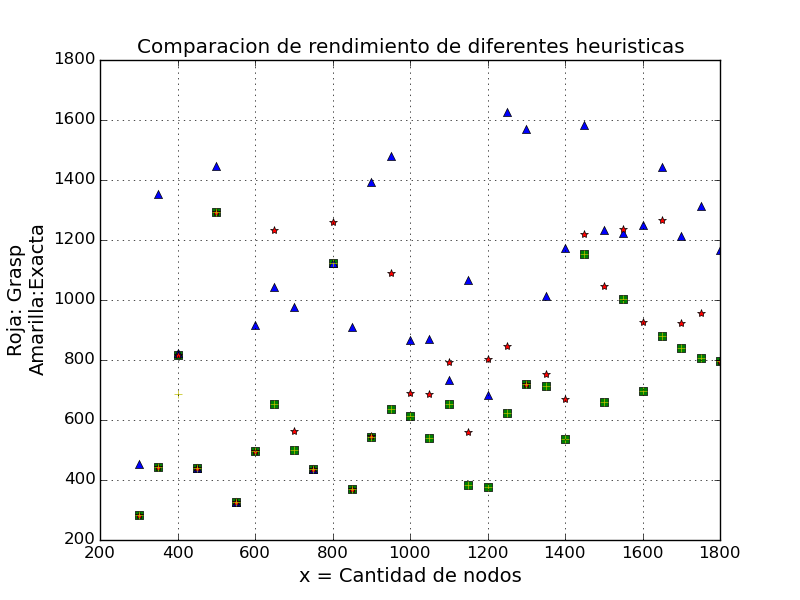
\includegraphics[scale=0.7]{experimentos/performance-optimalidad-lineales-beta_n_over_128/comparacion_optimalidad.png}
\end{center}

%--------------------------------------------------------------------------------------

\subsubsection{Grafos aleatorios de intermedia densidad de aristas}
\textbf{Parametros del experimento:}
\begin{itemize}
	\item Cantidad de tests realizados: 255
	\item Cantidad minima de nodos: 100
	\item Cantidad maxima de nodos: 600
	\item Rango peso $w_1$: [0..250]
	\item Rango peso $w_2$: [0..400]
	\item Cota de $w_1$: 200
	\item Cantidad minima de aristas: $ n * \sqrt n$
	\item Cantidad maxima de aristas: $ 5 * n * \sqrt n$
\end{itemize}

\vspace{1cm}

\textbf{Resultados del analisis (Golosa):}
\begin{lstlisting}[frame=single]	
	Tiempo promedio microsegundos heuristica: 2700.713
	Tiempo promedio microsegundos exacto: 6803.960
	Heuristica da la solucion optima: 86.666% de los casos
	Lejania promedio de la heuristica a la solucion optima: 2.590%
	Desv. estandar de la lejania entre las soluciones: 9.77461
	Minima lejania entre bqlocal y exacta: 0
	Maxima lejania entre bqlocal y exacta: 79.000%
\end{lstlisting}

\textbf{Resultados del analisis (Busqueda local):}
\begin{lstlisting}[frame=single]	
	Tiempo promedio microsegundos heuristica: 529.705
	Tiempo promedio microsegundos exacto: 6803.960
	Heuristica da la solucion optima: 10.588% de los casos
	Lejania promedio de la heuristica a la solucion optima: 726.246%
	Desv. estandar de la lejania entre las soluciones: 904.16
	Minima lejania entre bqlocal y exacta: 0
	Maxima lejania entre bqlocal y exacta: 5900.000%
\end{lstlisting}

\vspace{2cm}

\begin{center}	
	\textbf{Distribucion de los resultados}\\
	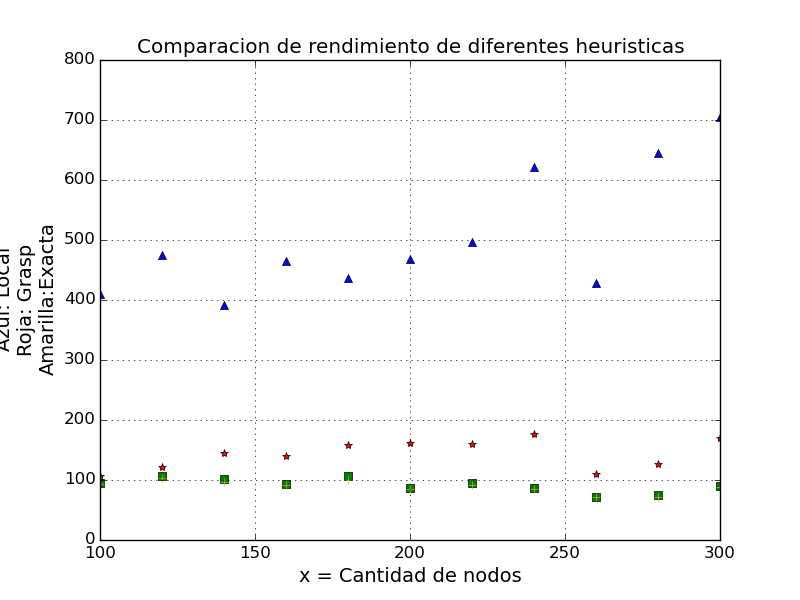
\includegraphics[scale=0.7]{experimentos/performance-optimalidad-intermedios/comparacion_optimalidad.png}
\end{center}

%--------------------------------------------------------------------------------------

\subsubsection{Grafos aleatorios de alta densidad de aristas}
\textbf{Parametros del experimento:}
\begin{itemize}
	\item Cantidad de grafos analizados: 53
	\item Cantidad minima de nodos: 10
	\item Cantidad maxima de nodos: 280
	\item Rango peso $w_1$: [0..250]
	\item Rango peso $w_2$: [0..400]
	\item Cota de $w_1$: 200
	\item Cantidad minima de aristas: $\frac{n * (n-1)}{3}$
	\item Cantidad maxima de aristas: $\frac{n * (n-1)}{2}$
\end{itemize}

\vspace{1cm}

\textbf{Resultados del analisis (Golosa):}
\begin{lstlisting}[frame=single]	
	Tiempo promedio microsegundos heuristica: 4569.584
	Tiempo promedio microsegundos exacto: 19571.283
	Heuristica da la solucion optima: 83.018% de los casos
	Lejania promedio de la heuristica a la solucion optima: 4.990%
	Desv. estandar de la lejania entre las soluciones: 18.1754
	Minima lejania entre bqlocal y exacta: 0
	Maxima lejania entre bqlocal y exacta: 110.300%
\end{lstlisting}

\textbf{Resultados del analisis (Busqueda local):}
\begin{lstlisting}[frame=single]	
	Tiempo promedio microsegundos heuristica: 550.485
	Tiempo promedio microsegundos exacto: 19571.283
	Heuristica da la solucion optima: 13.207% de los casos
	Lejania promedio de la heuristica a la solucion optima: 1042.275%
	Desv. estandar de la lejania entre las soluciones: 1153.29
	Minima lejania entre bqlocal y exacta: 0
	Maxima lejania entre bqlocal y exacta: 4473.000%
\end{lstlisting}

\vspace{2cm}

\begin{center}	
	\textbf{Distribucion de los resultados}\\
	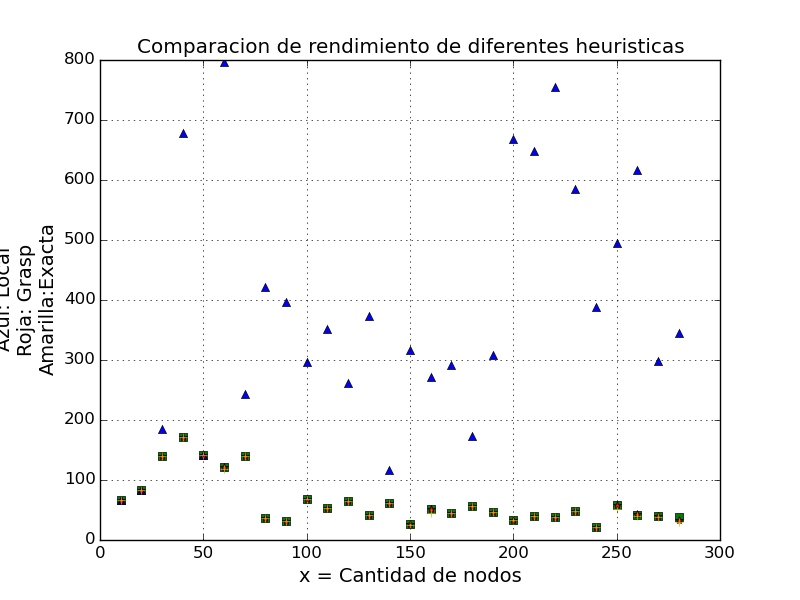
\includegraphics[scale=0.7]{experimentos/performance-optimalidad-cliques_beta_n_over_128/comparacion_optimalidad.png}
\end{center}


Conclusion: ??









\subsubsection{Metaheuristica GRASP - Variacion de parametros}

\subsection{Experimentacion pura entre heuristicas}
En esta secci\'on experimentaremos para varios conjuntos aleatorios de grafos de diferentes densidades con las heur\'isticas implementadas,sin tener en cuenta la soluci\'on exacta, para poder realizar experimentos con una mayor cantidad de nodos y aristas en las instancias. Dados los resultados, analizaremos de las 3 heur\'isticas implementadas cual obtiene en promedio y con que desviacion estandar, las soluciones con peso $w_2$ menor, y de esta forma, mas cercanas a la exacta.\\

Esto se realizara, para cada ejecucion de las 3 heuristicas, incrementando un contador en la que corresponda si su peso $w_2$ es minimo, al final tendremos, para cada heuristica, cuantas veces dio la minima solucion, y la cantidad total de instancias testeadas, con estos datos podremos realizar los analisis estadisticos.



3 familias de grafos, variando el beta si corresponde

lineal, cuadratico e intermedio, para el intermedio poner 
los calculos de porque la cuenta n(n-1)/x y n(n-1)/y es densidad intermedia para los valores de n entre k y j